\chapter{Domain} \label{cap:problem_domain}

In this chapter, we will delve into the details of melanoma cancer, including
its origins, factors contributing to its development, and strategies to
minimize the risk of its occurrence. Additionally, we will explore other common
types of skin cancer and their underlying causes. \\

By the end of this chapter, our aim is to provide a comprehensive understanding
of this condition, equipping you with the knowledge necessary to comprehend the
proposed solution in this thesis.

\section{The Skin}

The skin, which is our body's largest organ \cite{BaseCancerKnowledge}, plays a
crucial role in safeguarding us against external threats and maintaining our
overall health. It consists of several layers (Figure
\ref{fig:melanoma_diagram}), with the main layers being:

\begin{itemize} \item \textbf{Epidermis}

      The epidermis is the outermost layer of the skin, serving as a protective
      shield against environmental factors. It consists mainly of flat,
      scale-like cells called keratinocytes. These cells produce a tough
      protein called keratin, which helps make the skin waterproof and
      resistant to damage. Within the epidermis, specialized cells called
      melanocytes produce melanin, the pigment responsible for skin color.
      Melanin also helps protect the skin from harmful ultraviolet (UV)
      radiation. \\

      The epidermis is made up of several layers, including the stratum
      corneum, the topmost layer composed of dead skin cells that are
      continuously shed and replaced by new cells from the lower layers. The
      epidermis also contains other types of cells, such as Langerhans cells,
      which are part of the immune system and help defend against infections.

      \newpage

    \item \textbf{Dermis}

      Beneath the epidermis lies the dermis, a complex layer that provides
      structural support to the skin. The dermis contains a network of blood
      vessels that supply nutrients and oxygen to the skin cells. It also
      houses various structures, including hair follicles, sweat glands,
      sebaceous glands, and nerve endings. The dermis is composed of collagen
      and elastin fibers, which give the skin its strength, elasticity, and
      flexibility. These fibers allow the skin to stretch and recoil as needed.
      The dermis also plays a crucial role in thermoregulation by regulating
      blood flow to control body temperature.

    \item \textbf{Hypodermis (Subcutaneous Tissue)}

      The deepest layer of the skin is called the hypodermis or subcutaneous
      tissue. It is primarily made up of adipose tissue, which provides
      insulation, cushioning, and energy storage. The hypodermis helps to
      regulate body temperature by acting as an insulating layer, preventing
      heat loss. It also acts as a shock absorber, protecting the underlying
      structures and organs from injury. Additionally, the hypodermis serves as
      a connection between the skin and the underlying muscles and bones. It
      contains blood vessels and nerve endings that supply nutrients and
      sensations to the skin.

\end{itemize}

\begin{figure}[H] \centering
  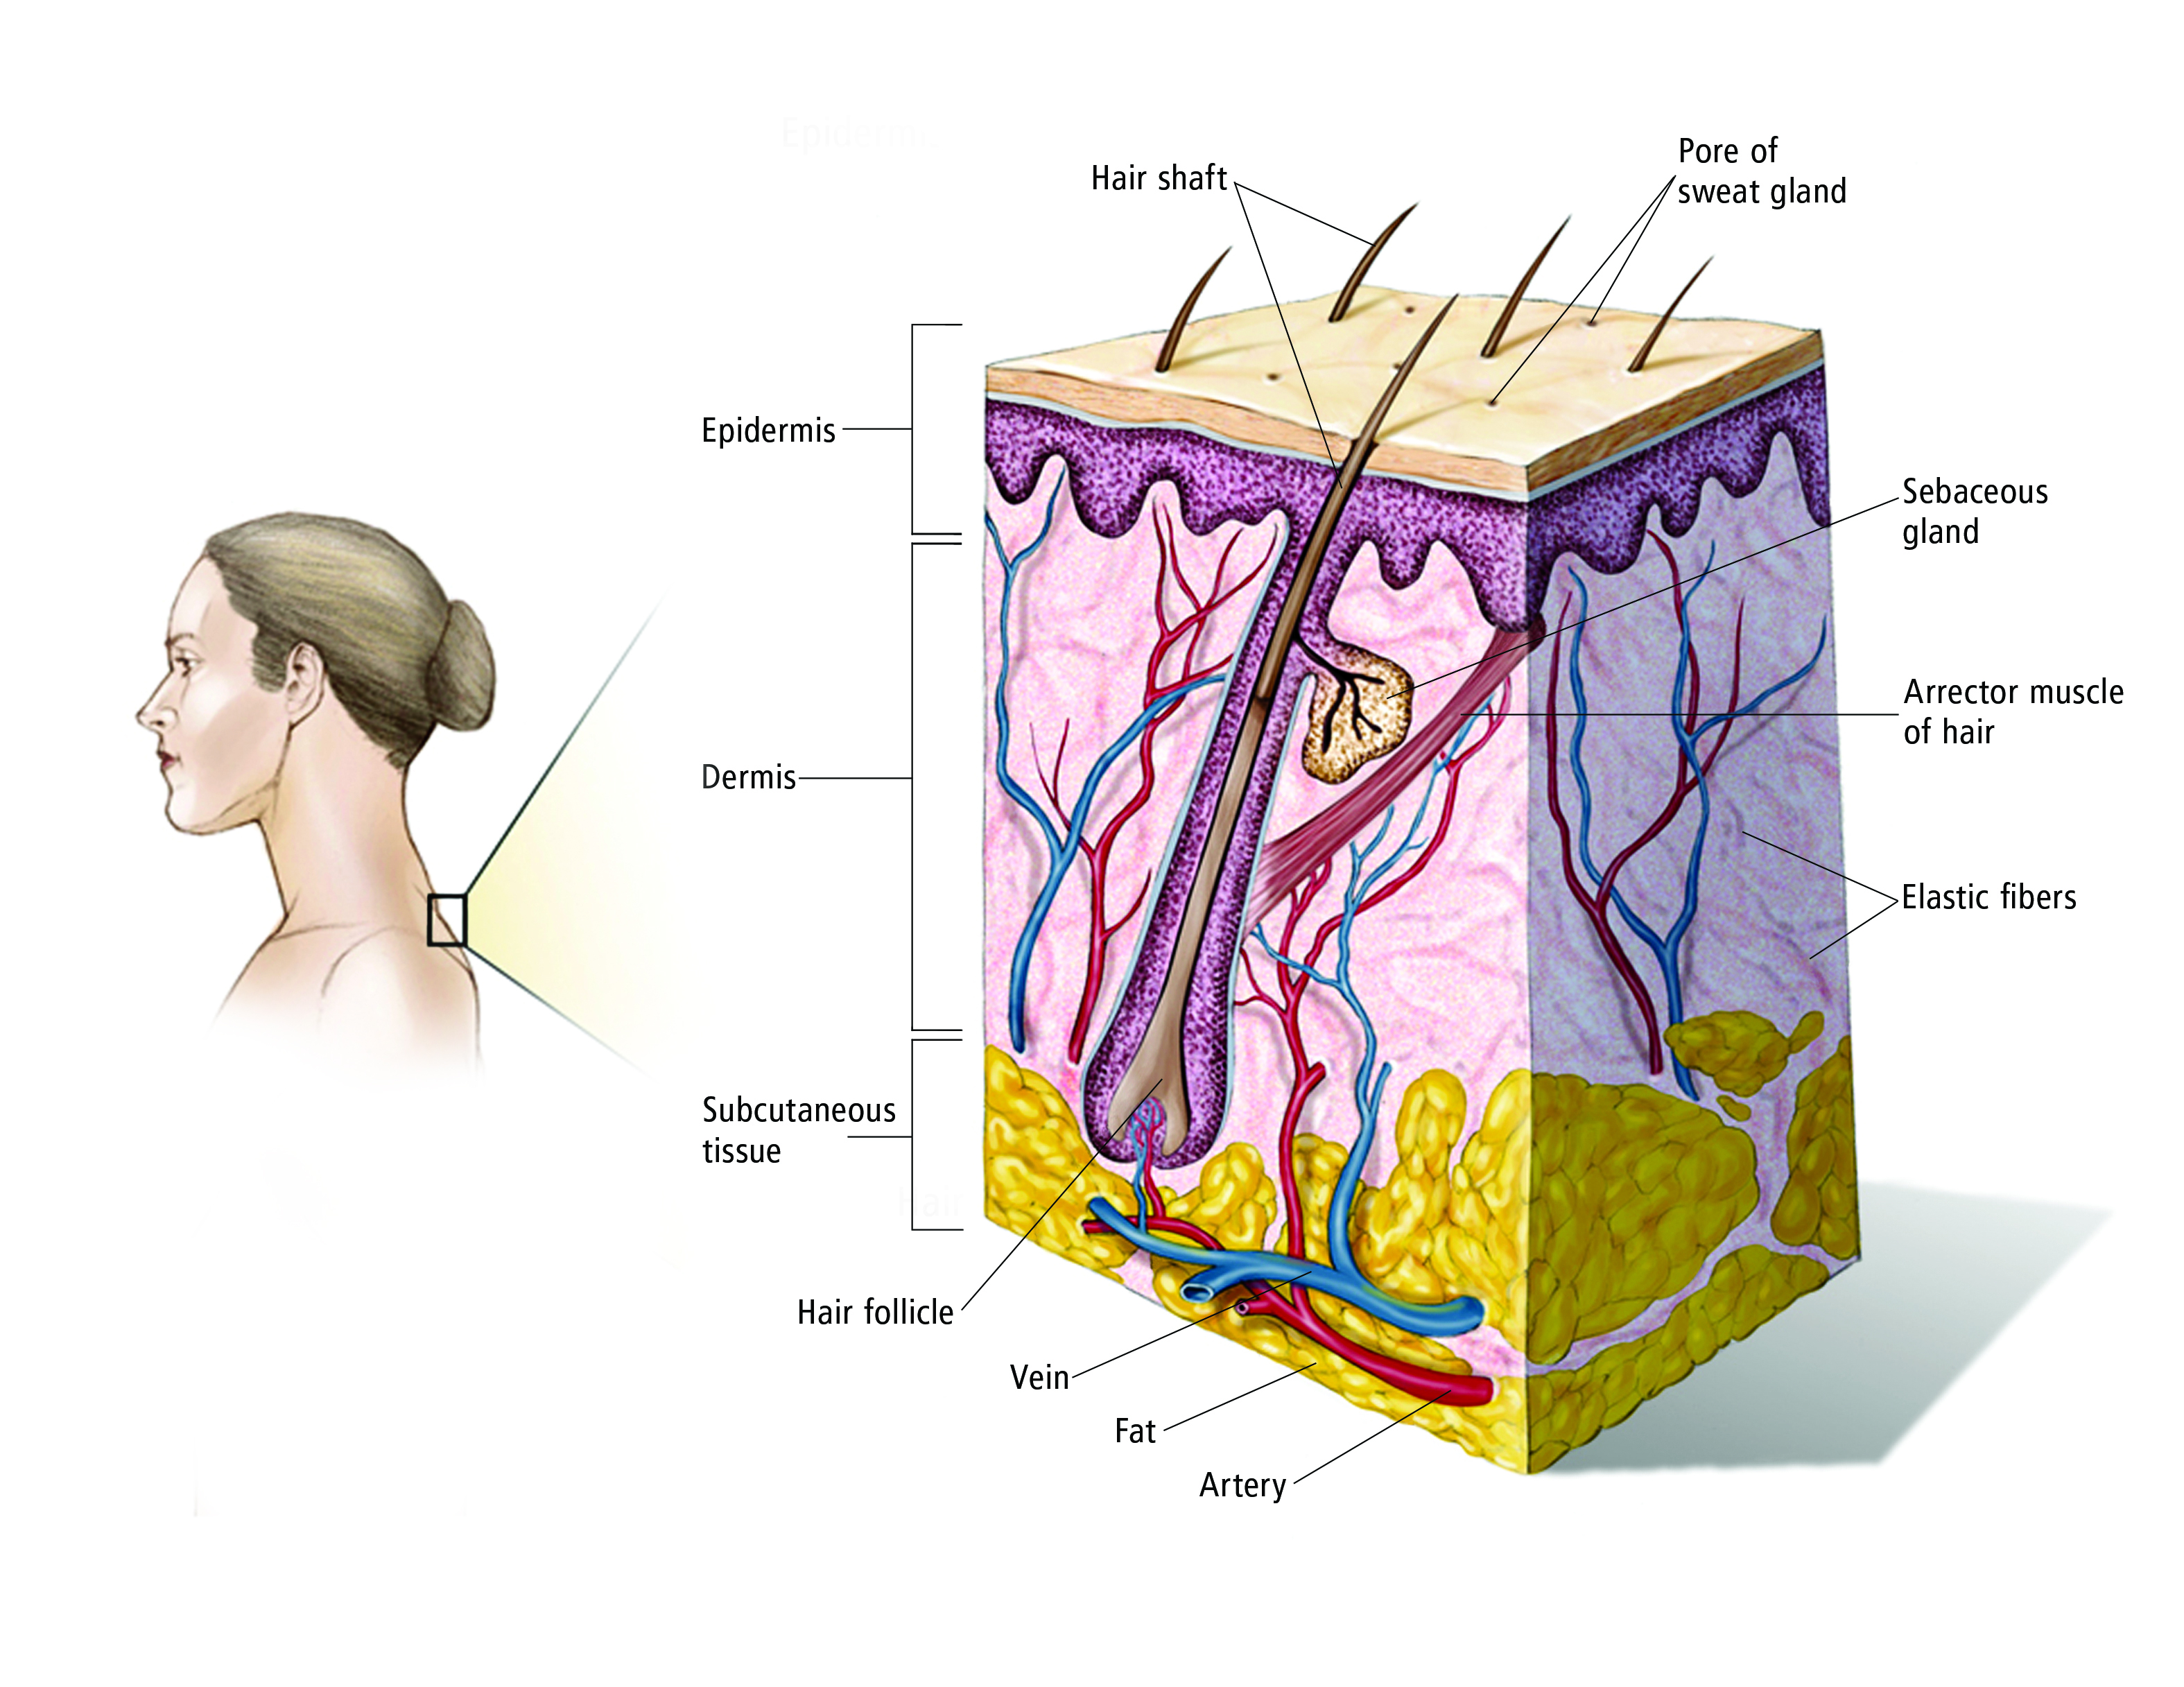
\includegraphics[width=0.85\textwidth]{imatges/problem_domain/melanoma-diagram.jpg}
  \caption[Skin Main Layers]{\textit{Skin Main Layers. Illustration by
Cancer.Net}} {\label{fig:melanoma_diagram}} \end{figure}

\section{Skin Cancer}

Cancer begins when healthy cells undergo changes that cause them to grow and
divide uncontrollably, forming a mass known as a tumor. Tumors can be
classified as either cancerous or benign. A cancerous tumor is considered
malignant, meaning it has the potential to invade nearby tissues and spread to
other parts of the body through a process called metastasis. Conversely, a
benign tumor may grow locally but does not have the ability to spread to other
areas. \\

Skin cancer is one of the most prevalent types of cancer, with over 3 million
Americans diagnosed each year. However, the prognosis for skin cancer is
generally favorable when detected early. Treatment options for skin cancer
often involve topical medications, in-office procedures performed by
dermatologists, or outpatient surgeries. Dermatologists specialize in
diagnosing and treating conditions of the skin. As a result, skin cancer
accounts for less than 1\% of all cancer-related deaths. \\

In more advanced cases, skin cancer may require comprehensive medical care
provided by a multidisciplinary team, which typically includes a dermatologist,
surgical oncologist, radiation oncologist, and clinical oncologist.

\subsection{Types of Skin Cancer}

There are three primary forms of skin cancer \cite{BaseCancerKnowledge}.

\begin{itemize}

  \item \textbf{Basal cell carcinoma}

    This type of skin cancer arises from basal cells located in the lower
    epidermis. Approximately 80\% to 90\% of skin cancers originate from
    these cells, leading to the designation of basal cell carcinomas. They
    typically develop on the head and neck, although they can occur anywhere
    on the skin. Sun exposure is the primary cause, although they may also
    occur in individuals who underwent radiation therapy during childhood.
    This type of skin cancer generally grows slowly and rarely metastasizes
    to other parts of the body.

  \item \textbf{Squamous cell carcinoma}

    This type of skin cancer originates from flat, scale-like cells known as
    squamous cells that comprise a significant portion of the epidermis.
    Around 10\% to 20\% of skin cancers develop from these cells, resulting
    in the classification of squamous cell carcinomas. Sun exposure is the
    main cause, and they can be diagnosed on various regions of the skin.
    They may also emerge on skin that has been burned, damaged by chemicals,
    or exposed to x-rays. Common sites for squamous cell carcinoma include
    the lips, areas with long-standing scars, and the skin surrounding the
    mouth, anus, and vagina. Roughly 2\% to 5\% of squamous cell carcinomas
    metastasize to other parts of the body.

  \item \textbf{Melanoma}

    The most aggressive type of skin cancer, originates in scattered cells
    known as melanocytes where the epidermis and dermis meet. Melanocytes
    produce the pigment melanin, responsible for skin color. Melanoma
    accounts for approximately 1\% of all skin cancers.

\end{itemize}

\subsection{Stages}

The following stages are used for basal cell carcinoma and for squamous cell
cancer. The stages consist in a slow-growing cancer that seldom spreads to
other parts of the body \cite{CancerInstitute}. \\

\begin{itemize}

  \item \textbf{Stage 0}

    In stage 0, abnormal cells are found in the squamous cell or basal cell
    layer of the epidermis. These abnormal cells may become cancer and spread
    into nearby normal tissue.

    \begin{figure}[H] \centering
      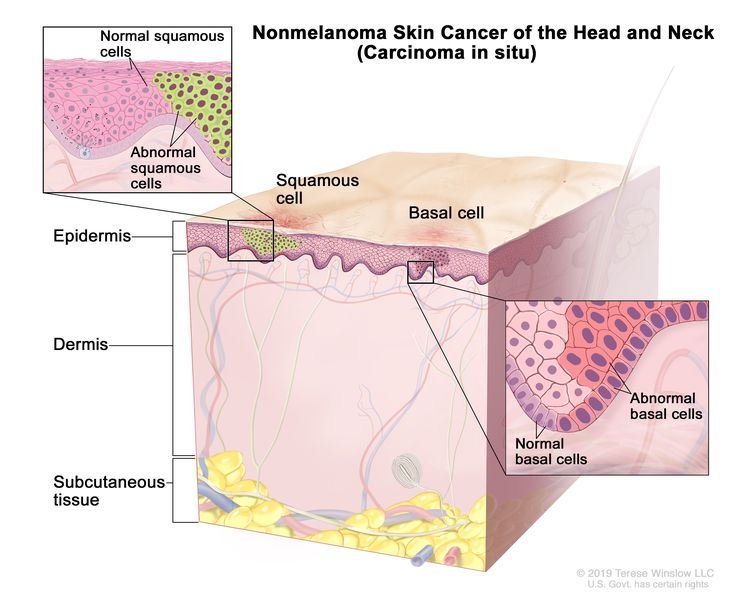
\includegraphics[width=0.6\textwidth]{imatges/problem_domain/phase0-skin-cancer.jpg}
      \caption[Skin Cancer, Stage 0]{\textit{Skin Cancer, Stage 0. Illustration by Terese Winslow}}
    {\label{fig:stage0-skin-canceer}} \end{figure}

    \newpage


  \item \textbf{Stage I}

    In stage I, cancer has formed and the tumor is 2 centimeters or smaller.

    \begin{figure}[H] \centering
      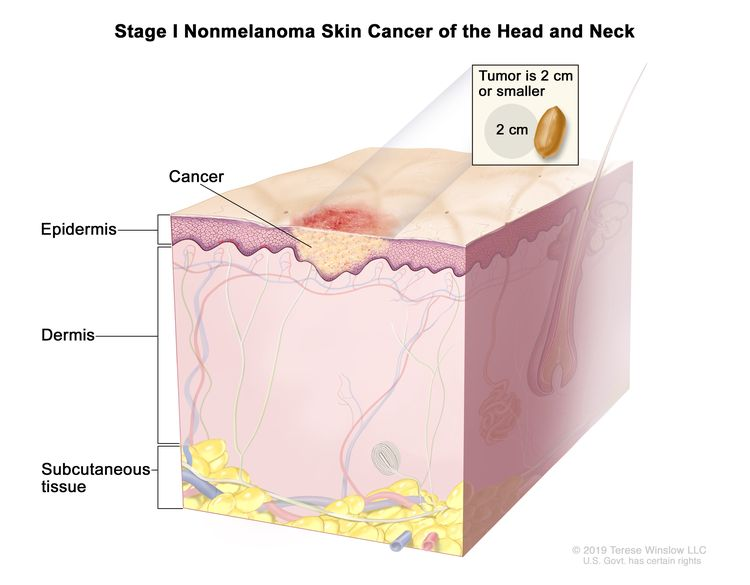
\includegraphics[width=0.6\textwidth]{imatges/problem_domain/stage1-skin-cancer.jpg}
      \caption[Skin Cancer, Stage I]{\textit{Skin Cancer, Stage I.
      Illustration by Terese Winslow}} {\label{fig:stage1-skin-canceer}}
    \end{figure}


  \item \textbf{Stage II}

    In stage II, the tumor is larger than 2 centimeters but not larger than 4
    centimeters.

    \begin{figure}[H] \centering
      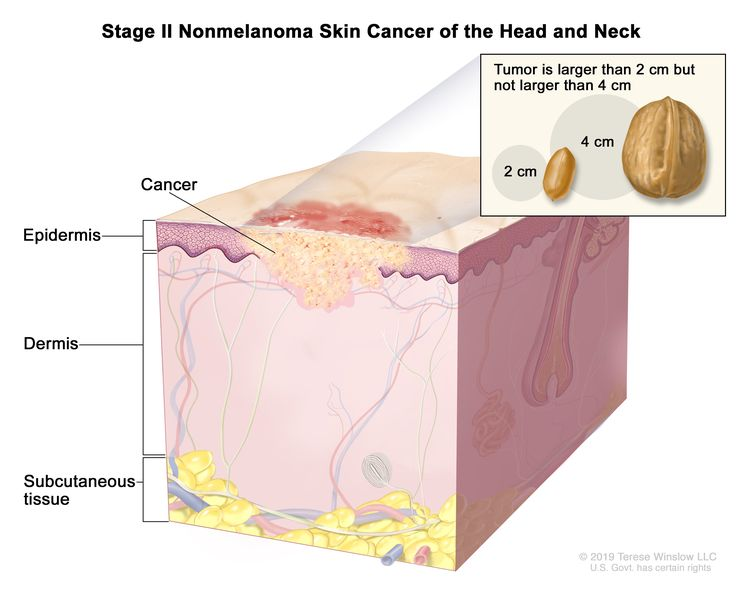
\includegraphics[width=0.6\textwidth]{imatges/problem_domain/stage2-skin-cancer.jpg}
      \caption[Skin Cancer, Stage II]{\textit{Skin Cancer, Stage II.
      Illustration by Terese Winslow}} {\label{fig:stage2-skin-canceer}}
    \end{figure}

    \newpage

  \item \textbf{Stage III}

    In this stage, the cancer may spread to the rest of the body covering the
    nerves bellow the dermis or bellow the subcutaneous tissue or the bones.

    \begin{figure}[H] \centering
      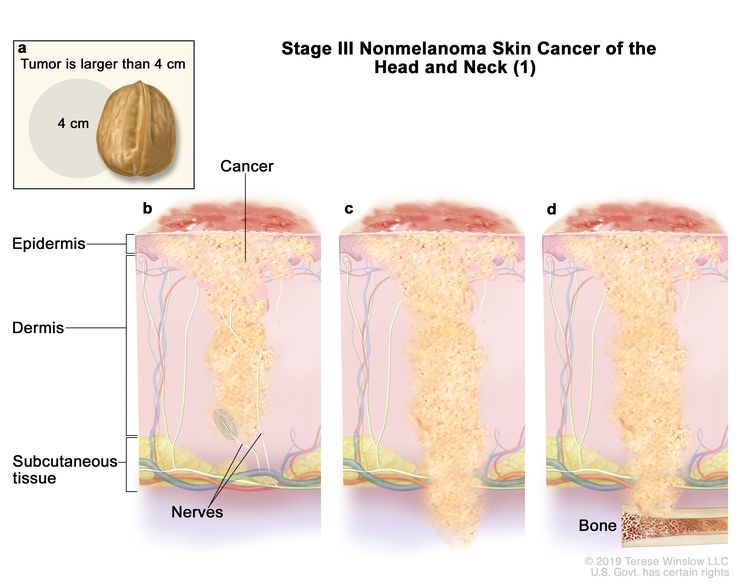
\includegraphics[width=0.6\textwidth]{imatges/problem_domain/stage3-skin-cancer.jpg}
      \caption[Skin Cancer, Stage III]{\textit{Skin Cancer, Stage III. Illustration by
    Terese Winslow}} {\label{fig:stage3-skin-canceer}} \end{figure}

\end{itemize}

\subsection{Associated Factors and Prevention of Skin Cancer}

The risk factors associated with skin cancer encompass sun exposure, fair skin,
as well as certain physical characteristics such as blond hair and blue eyes.
The presence of melanin, a protein responsible for the skin's color or pigment,
plays a crucial role in shielding the skin from ultraviolet (UV) radiation.
Consequently, individuals with lighter skin or lower levels of melanin possess
reduced UV protection \cite{OrigenAndTreatment}. \\

Although skin cancer may initially appear to predominantly affect individuals
with light complexions, those with dark skin are also susceptible. They may
observe signs of cancer on the palms of their hands or soles of their feet.
\\

Advancements in research have led to treatments targeting the genetic level.
New drug therapies assist in stimulating the immune system to produce
antibodies capable of combatting rapidly dividing cells. While these therapies
may have potential side effects, they are generally milder than those
associated with chemotherapy. Moreover, they result in an enhanced immune
system that is better equipped to fight cancer. \\

A patient's overall health also appears to influence their ability to fight
cancer, although the precise connection between one's health and their risk of
developing cancer remains unclear. However, it can be assumed that better
overall health enhances the immune system's capacity to combat cancer. \\

Prevention of skin cancer is straightforward: minimizing exposure to the sun
and UV radiation. Ceasing the use of tanning beds is advised. When exposed to
the sun, wearing sunscreen and a wide-brimmed hat that provides comprehensive
head shading is recommended \cite{OrigenAndTreatment}. \\

Consideration should also be given to wearing clothing with SPF\footnote{Sun
Protection Factor} protection. Some clothing manufacturers now produce summer
attire with SPF levels similar to those found in sunscreen. This is significant
since most regular t-shirts offer only minimal SPF protection of around 2. \\

Skin cancer ranks among the most prevalent forms of cancer, yet it is also one
of the most easily detectable and treatable. Taking proactive measures to
prevent sun exposure is crucial, while early detection is highly important. The
prognosis is favorable when melanoma is identified in its early stages.
